\documentclass[border=8pt]{standalone}
\usepackage{pgfplots}
\usetikzlibrary{arrows.meta}
\pgfplotsset{compat=1.18}
\begin{document}
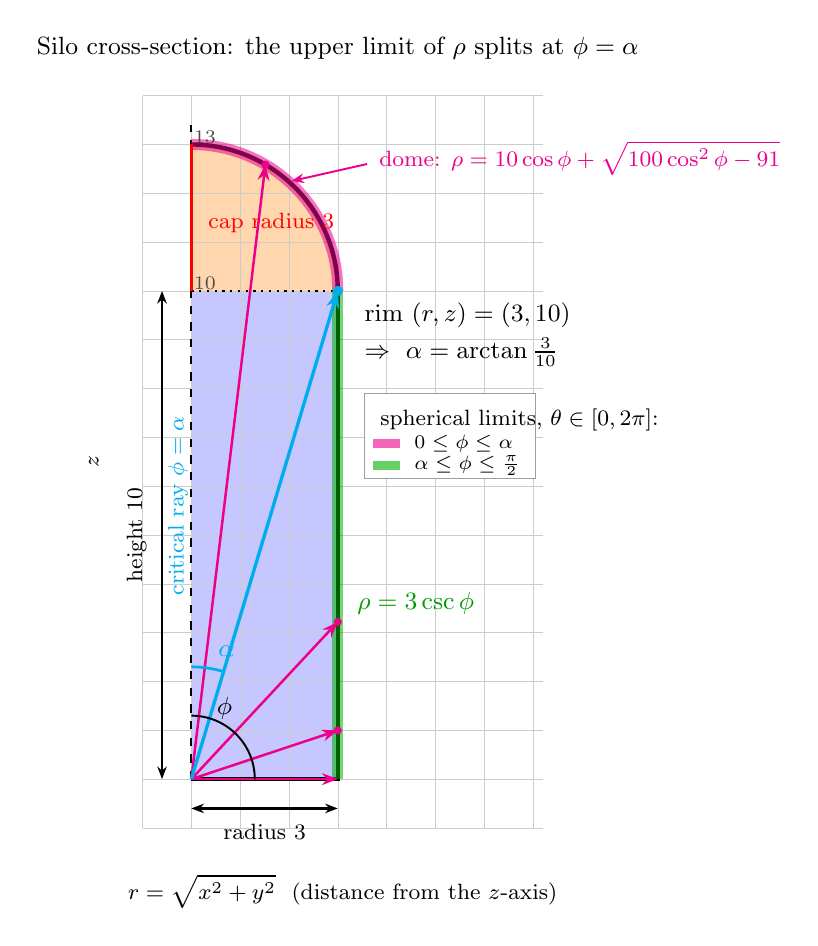
\begin{tikzpicture}[scale=0.62]
% ---------------- shaded interior (dome: arc of radius 3 about (0,10)) --------
\fill[blue!22] (0,0) rectangle (3,10);
\fill[orange!32] (0,10) -- (3,10) arc (0:90:3) -- cycle;

% ---------------- grid / guides ----------------
\draw[help lines,color=black!20] (-1,-1) grid (7.2,14);
\draw[dashed,thick] (0,0) -- (0,13.4);          % axis of revolution
\draw[dotted,thick] (0,10) -- (3,10);           % seam z = 10

% ---------------- outline of the silo ----------------
\draw[ultra thick] (0,0) -- (3,0) -- (3,10);
\draw[ultra thick] (3,10) arc (0:90:3);

% ---------------- the two rho-boundaries, highlighted ----------------
\draw[magenta,line width=1.4mm,opacity=.55] (3,10) arc (0:90:3);
\draw[green!70!black,line width=1.4mm,opacity=.55] (3,0) -- (3,10);

% ---------------- rays from the origin ----------------
\draw[-{Stealth[length=2mm]},magenta,line width=0.9pt] (0,0) -- (1.5178,12.5877);
\draw[-{Stealth[length=2mm]},magenta,line width=0.9pt] (0,0) -- (3,3.2203);
\draw[-{Stealth[length=2mm]},magenta,line width=0.9pt] (0,0) -- (3,0.9968);
\draw[-{Stealth[length=2mm]},magenta,line width=0.9pt] (0,0) -- (3,0);
\fill[magenta] (1.5178,12.5877) circle (2.4pt);
\fill[magenta] (3,3.2203) circle (2.4pt);
\fill[magenta] (3,0.9968) circle (2.4pt);
% critical ray  phi = alpha = arctan(3/10)
\draw[-{Stealth[length=2.2mm]},cyan,line width=1.2pt] (0,0) -- (3,10);
\fill[cyan] (3,10) circle (3pt);

% ---------------- angle arcs ----------------
\draw[cyan,line width=1pt] (0,2.3) arc (90:73.301:2.3);
\draw[line width=0.7pt] (0,1.3) arc (90:0:1.3);
\node[cyan,font=\small] at (0.72,2.62) {$\alpha$};
\node[font=\small] at (0.68,1.45) {$\phi$};
\node[cyan,rotate=90,font=\footnotesize,anchor=south] at (0.13,5.6) {critical ray $\phi=\alpha$};

% ---------------- dimensions ----------------
\draw[{Stealth[length=1.6mm]}-{Stealth[length=1.6mm]},line width=0.8pt] (0,-0.6) -- (3,-0.6);
\node[font=\footnotesize,anchor=north] at (1.5,-0.72) {radius 3};
\draw[{Stealth[length=1.6mm]}-{Stealth[length=1.6mm]},line width=0.8pt] (-0.6,0) -- (-0.6,10);
\node[font=\footnotesize,rotate=90,anchor=south] at (-0.72,5.0) {height 10};
\draw[red,line width=1.2pt] (0,10) -- (0,13);
\node[red,font=\footnotesize,anchor=west] at (0.15,11.4) {cap radius 3};
\node[font=\scriptsize,text=black!70] at (0.28,13.15) {$13$};
\node[font=\scriptsize,text=black!70] at (0.28,10.15) {$10$};

% ---------------- right-hand annotations ----------------
\node[below right,font=\small,text=black,align=left] at (3.35,9.95)
     {rim $(r,z)=(3,10)$};
\node[below right,font=\small,text=black,align=left] at (3.35,9.25)
     {$\Rightarrow\ \alpha=\arctan\frac{3}{10}$};
\draw[-{Stealth[length=1.6mm]},magenta,line width=0.7pt] (3.6,12.6) -- (2.05,12.25);
\node[magenta,font=\footnotesize,anchor=west,align=left,text=magenta] at (3.65,12.72)
     {dome: $\rho=10\cos\phi+\sqrt{100\cos^2\phi-91}$};
\node[green!60!black,font=\small,anchor=west] at (3.2,3.6) {$\rho=3\csc\phi$};

% ---------------- legend ----------------
\begin{scope}[shift={(3.55,7.9)}]
 \draw[fill=white,opacity=.96,draw=black!40] (0,0) rectangle (3.5,-1.75);
 \node[font=\footnotesize,anchor=north west,text=black,align=left] at (0.12,-0.12)
      {spherical limits, $\theta\in[0,2\pi]$:};
 \draw[magenta,line width=1.2mm,opacity=.6] (0.18,-1.02) -- (0.72,-1.02);
 \node[font=\scriptsize,anchor=west,text=black] at (0.82,-1.02) {$0\le\phi\le\alpha$};
 \draw[green!70!black,line width=1.2mm,opacity=.6] (0.18,-1.48) -- (0.72,-1.48);
 \node[font=\scriptsize,anchor=west,text=black] at (0.82,-1.48) {$\alpha\le\phi\le\frac{\pi}{2}$};
\end{scope}

% ---------------- frame labels ----------------
\node[font=\footnotesize,anchor=north] at (3.1,-1.75)
  {$r=\sqrt{x^2+y^2}$\ \ (distance from the $z$-axis)};
\node[font=\footnotesize,rotate=90,anchor=south] at (-1.7,6.5) {$z$};
\node[font=\small,anchor=south] at (3.0,14.55)
  {Silo cross-section: the upper limit of $\rho$ splits at $\phi=\alpha$};
\end{tikzpicture}
\end{document}
